\section{Feature aggregation}

Information derived from counts of linguistic features in texts can be used in various ways for characterizing the the texts they were extracted from. In pioneering work by \cite{Biber1988},
 \cite{Biber1995}, factor analysis was used to identify a number of ``dimensions of variation'' that could be interpreted in terms of communicative function (such as ``narrative vs.\ non-narrative'', ``involved vs.\ informational production''), and individual texts can then be located at different points on each one of these scales. Contrasting with this multidimensional approach, there have also been attempts to automatically assign texts to single a category (``genre'', ``text type'') based on the occurrence of linguistic features on those texts. An early example of such an approach is \cite{KarlgrenCutting1994}. A recent state-of-the-art example is reported in \cite{EgbertBiberDavis2015}, which illustrates the enormous challenge of automatic register classification on the basis of linguistic feature counts. Using 44 linguistic features in a discriminant analysis for predicting the register category of documents from an ``unrestricted corpus of web documents'', they report precision = 0.342 and recall = 0.396 for their 20 specific sub-registers used in the task (results are generally lower when a smaller number of broader, less specific register categories is used).

In order to explore the effects of feature aggregation in predicting potentially register-sensitive morpho-syntactic alternation phenomena, we use a multidimensional approach (based on Factor Analysis) as described in \cite{Biber1988,Biber1995}. 
In Section~\ref{sec:case-studies}, we will treat the documents' factor scores on each one of the resulting factors as document meta data, and use that meta data in modeling the outcome in specific instances of the alternation phenomenon.
Note that in using a multidimensional approach, we still produce several document-level predictors.
In contrast, assigning each document to a single register category would produce only a single document-level predictor, leading to a greater loss of information.  


\subsection{Factor analysis}

In general, we sought to reproduce the technical aspects of Biber's (1988) study as closely as possible.
There is a major difference, however, in corpus size.
While Biber used material from a total of 481 documents, %(comprising 960,000 words)
 we sampled 70,000 documents from DeReKo and DECOW16B each, totaling 140,000 documents.
Another difference concerns document length.
\cite{Biber1988} imposes an upper limit of approximately 2,500 words per document, whereas we base our counts on whole documents, without an upper limit to the number of words.
The minimum text length is 400 words in Biber's study.
In contrast, we use a lower threshold of only 100 tokens (many documents DeReKo are actually shorter than that).

For the factor analysis, we used a total of 60 feature counts extracted with COReX.\footnote{Absolute counts, such as number of tokens and number of sentences, were discarded.}
The \textit{genitive} count, originally extracted by COReX, was discarded in view of the case study reported in Section~\ref{sec:case-studies}, where the occurrence of genitive is predicted.
 All normalized counts were scaled to z-scores.
 Visual inspection of a parallel analysis scree plot suggested an optimal number of 7 to 8 factors for our data set.
 The plot in Figure~\ref{fa-pa-7-factors} shows the factor loadings from a factor analysis using 7 factors.
 The factoring and rotation methods (\textit{principal factor} and \textit{promax}, respectively) were chosen to match those used and recommended in \cite{Biber1988}.
 
 
\begin{figure}
   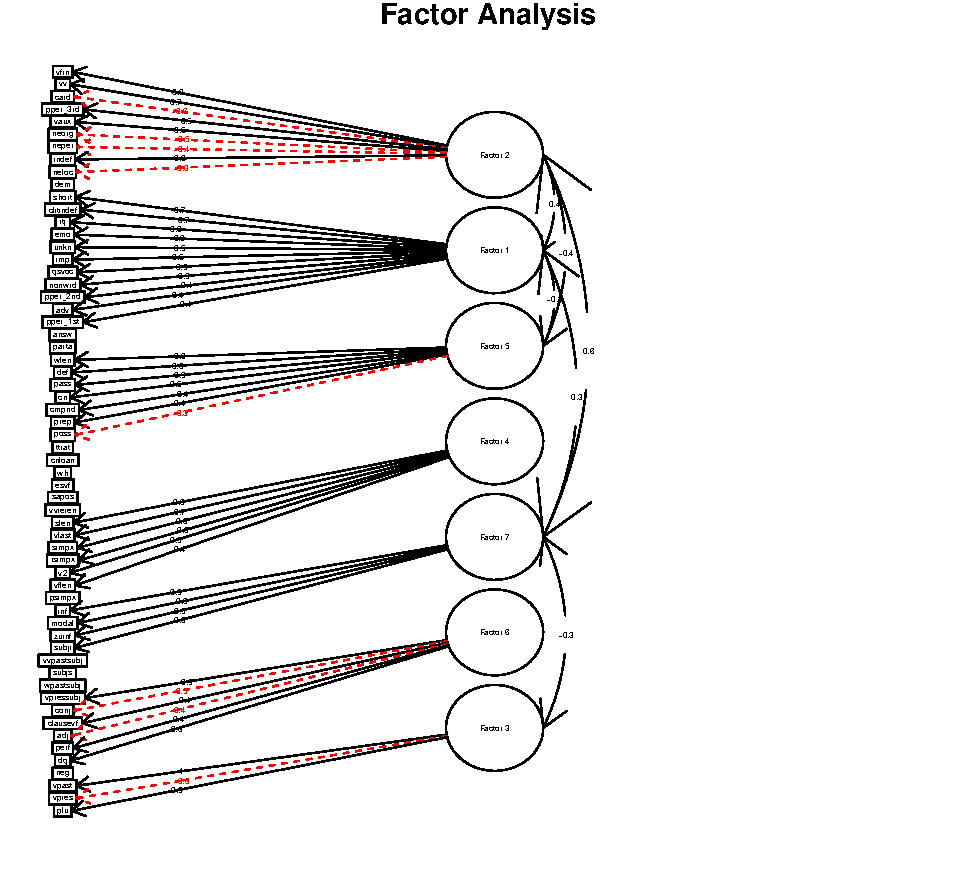
\includegraphics[scale=.9]{../R/plots/fa-fa-7-promax-padded}
   \label{fa-pa-7-factors}
  \caption{Factor loadings of 60 COReX features, from a factor analysis of 140.000 randomly selected documents (DeReKo and DECOW16 combined, minimal document length = 100 tokens), 7 factors, principal factor method, promax rotation. Only the highest factor loading is shown for each feature (loadings between $-0.35$ and $0.35$ are omitted).}  
\end{figure}



Some, but not all of the factors lend themselves to an interpretation in terms of meaningful dimensions of variation.
Most notable among these is Factor~1.
Features with high factor loadings on Factor~1 include short/ contracted forms, interjections, emoticons, imperatives, vocabulary typical of informal written language, as well as first and second person pronouns.
Factor~1 thus most probably captures variability along the lines of formal vs.\ informal, standard vs.\ non-standard, high vs.\ low degree of interaction.
On closer inspection of a number of documents with high scores on Factor~1, it turned out that ``non-standard'' also extends to dialectal texts.
In contrast, finding a plausible interpretation for factors such as Factor~2 is not as straightforward.
Features positively associated with Factor~2 include finite verbs, lexical verbs, auxiliary verbs and third person pronouns, while a significant number of features are negatively associated with it (including cardinal numbers and various types of named entities).

Factor scores were computed for every factor for each one of the 140,000 documents in the sample, along the lines of \cite{Biber1988}, p.\,93--97, as follows:

\begin{itemize}
  \item Factor loadings whose absolute value is less than 0.35 were ignored.
  \item Any given feature is part of only one factor (the one with the greatest loading for that feature).
  \item For each document, for each factor, standardized counts (i.\,e., z-scores) were added up for those features that are salient on that factor (salient meaning the feature's absolute loading is at least .35 and there is no other factor where this feature has a greater absolute loading).
\end{itemize}

This approach implies that the exact magnitude of a feature's  loading on a factor is irrelevant for the calculation of a document's factor scores; for instance, it does not make a difference whether a loading is .35 or .99.
%The only condition is that the feature must not be more salient on another factor.

\cite{Biber1988} proceeds by comparing the mean factor scores of documents belonging to different (externally defined) registers (such as \textit{romantic fiction}, \textit{biographies}, \textit{press reviews}) on various dimensions of variation (= interpreted factors).
Unfortunately, as was discussed above, the corpora used in our study hardly contain any reliable register information at all.
One distinction that can be made, though, is between texts from internet discussion forums (recognizable by their URL patterns) and any texts (web or other) that are not forum discussions.
We would expect forum discussions to exhibit a high degree of interaction (question/comment - reaction/answer), as well as a fair amount of non-redacted, non-standard language, and this is indeed what we find when we compare the distribution of document scores on Factor~1 for forum (mean 14.6) and non-forum (mean -1.3) documents, as shown in Figure~\ref{forum-factor1}.

\begin{figure}
   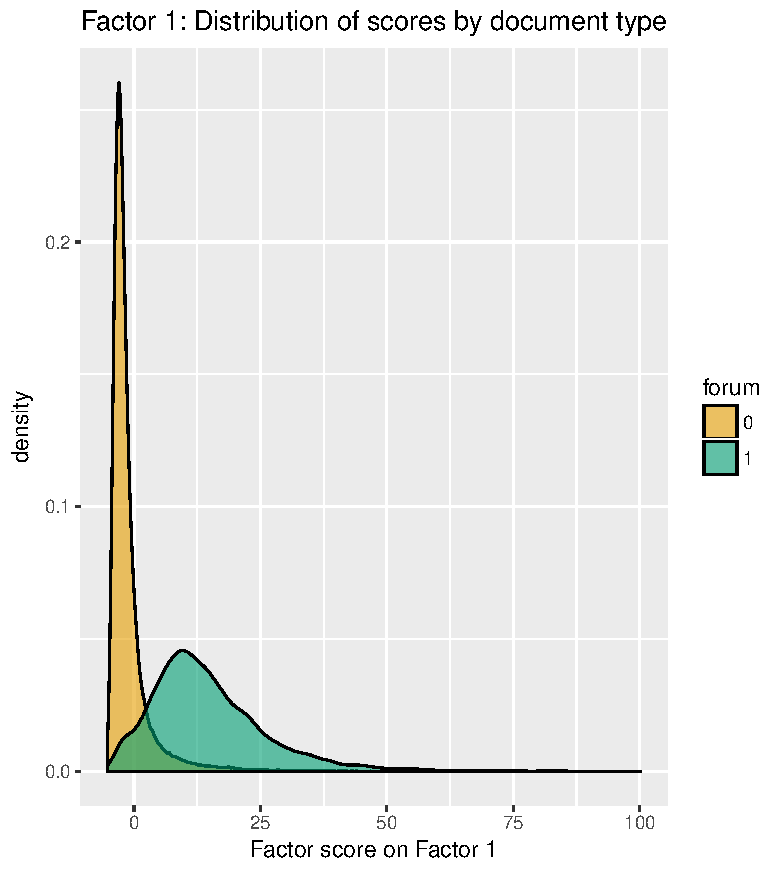
\includegraphics[scale=.95]{../R/plots/forum-factor1.pdf}
   \label{forum-factor1}
  \caption{Distribution of factor scores (Factor~1). On average, forum documents show higher scores (14.6) than non-forum documents ($-$1.3). Prominent features on Factor~1 include short/contracted word forms, cliticised variants of the indefinite article, interjections, imperatives, 1st and 2nd person pronouns, emoticons, and words typical of informal written language.}  
\end{figure}

By generating factor scores for each of the 7 factors for each document, we have enriched our corpus with 7 additional meta data variables at the document level.
In the next section, we will use these variables as document-level predictors in a study on a specific syntactic alternation phenomenon, and compare the results to alternative models that use non-aggregated COReX counts as predictors.





